%! Author = giaco
%! Date = 16/05/2024

\chapter{Background}
\label{sec:background}
In this chapter, we provide a brief overview of the main concepts that are necessary to understand the work presented in this thesis.
First of all, we start by introducing the concept of Machine Learning (ML) and Deep Learning (DL) in~\ref{sec:machine_learning}.
Then, in~\ref{sec:rl} we will talk in depth about one specific kind of learning, i.e.\ Reinforcement Learning, which is instead the main focus of this work, and we will talk also about Deep Reinforcement Learning (DRL).

\section{Machine Learning}
\label{sec:machine_learning}
%inserire immagine AI-ML-DL
% prendi immagini da qui https://www.geeksforgeeks.org/types-of-machine-learning/

Machine Learning, Fig. \ref{fig:ml_hierarchy}, is the branch of Artificial Intelligence that focuses on developing models and algorithms that let computers learn from data and improve from previous experience without being explicitly programmed for every task.
In simple words, ML teaches the systems to think and understand like humans by learning from the data.
ML finds application in many fields, including natural language processing, computer vision, speech recognition, email filtering, medicine, and many more

There are several types of ML family of algorithms, each with its own characteristics and applications.
Some of the main types are Supervised Learning, Unsupervised Learning, Self-Supervised Learning, and finally Reinforcement Learning, Fig.\ref{fig:ml_types}
A subset of ML is Deep Learning, which focuses on training neural networks with many layers.

We will talk about the different kinds of learning algorithms and DL in the following subsection, while since RL is the focus of this work we will dedicate a proper section.





\begin{figure}[ht]
    \begin{subfigure}[b]{0.45\textwidth}
        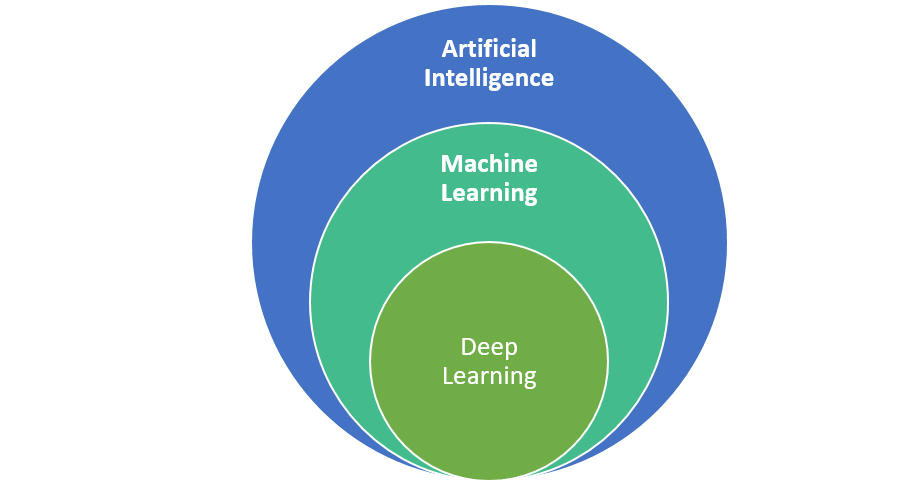
\includegraphics[width=\textwidth]{images/background/ai_ml_dl}
        \caption{\texttt{Artificial Intelligence hierarchy.}}
        \label{fig:ml_hierarchy}
    \end{subfigure}
    \hfill
    \begin{subfigure}[b]{0.45\textwidth}
        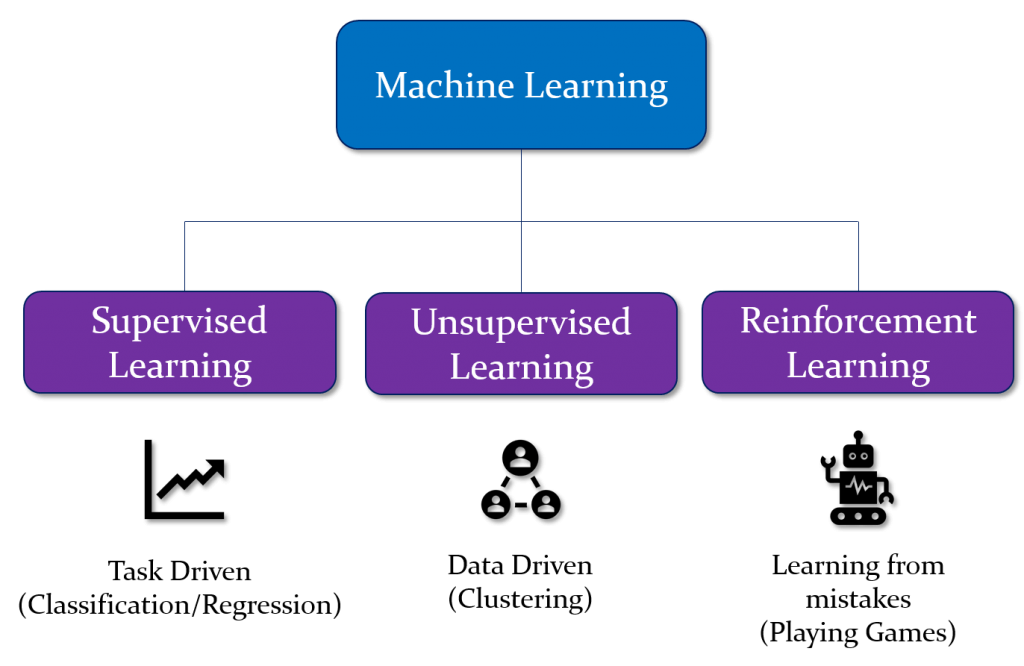
\includegraphics[width=\textwidth]{images/background/ML_Types}
        \caption{\texttt{Some Families of ML algorithms.}}
        \label{fig:ml_types}
    \end{subfigure}
    \hfill
    
\end{figure}








\subsubsection{Supervised Learning}
\label{subsubsec:supervised_ml}
%insert citation of examples of supervised learning?
Supervised Learning is a type of ML where the model is trained on a labeled dataset.
In this context, \textit{labeled} means that each training example is paired with an output label.
The goal of supervised learning is to learn a mapping from inputs to outputs that can be used to predict the output for new, unseen inputs.


There are two main categories of supervised learning that are:
\begin{itemize}
    \item Classification - The goal is to predict a discrete label.
    For example, classifying emails as spam or not spam, or recognizing handwritten digits.
    Classification algorithms learn to map the input features to one of the predefined classes.

    \item Regression - The goal is to predict a continuous value.
    For example, predicting the price of a house given its features, or the temperature for a given day.
    Regression algorithms learn to map the input features to a continuous numerical value.

\end{itemize}

%advantages and disadvantages
Supervised Learning models can have high accuracy as they are trained on labeled data. Also, they can be used as pre-trained models, which saves time and resources when developing new models from scratch.
They have some limitations though, in fact, sometimes they need a huge amount of data to perform well and they may struggle with unseen or unexpected patterns that are not present in the training data. Finally, they can be time-consuming when in the presence of a huge amount of data in the training set.

\subsubsection{Unsupervised Learning}
\label{subsubsec:unsupervised_ml}
Unsupervised learning is a type of ML technique in which an algorithm discovers patterns and relationships using unlabeled data.
Unlike supervised learning, unsupervised learning doesn’t involve providing the algorithm with labeled target outputs.
The primary goal of Unsupervised learning is often to discover hidden patterns, similarities, or clusters within the data, which can then be used for various purposes, such as data exploration, visualization, dimensionality reduction, and more.


The main categories of unsupervised learning are:
\begin{itemize}
    \item Clustering - This is the process of grouping data points into clusters based on their similarities.

    \item Association Rule learning - It is a method used for finding relationships between variables in a large database. A typical example of the Association Rule is the Market Basket Analysis which determines the set of items that occur together like people who buy a specific item also tend to purchase another item.

\end{itemize}


%advantages and disadvantages
Unsupervised Learning helps discover hidden patterns and relationships when labels for data are not available.
Without using labels though, it may be difficult to predict the quality of the model's output.





\subsubsection{Self-Supervised Machine Learning}
\label{sec:semisupervised_ml}
Self-supervised learning is a type of ML technique that falls in between supervised and unsupervised learning.
When in presence of a large amount of unlabeled data, self-supervised learning can be used to learn useful representations of the data.
In fact, it consists of pre-training a model using unlabelled data and generating data labels automatically. Then in the second phase, the algorithm uses the high-confidence data labels among those generated to train the model again in subsequent iterations, like the supervised learning method. The only difference is that the data labels used as ground truth in every iteration are changed.

Self-supervised learning is a powerful technique that can be used to learn useful representations of the data, and it can be used as a pre-training step for supervised learning tasks.
Self-supervised learning models were used in the development of this thesis as we will see in section INSERT.



\subsubsection{Deep Learning}
\label{sec:dl}
is a subfield of ML that, in the last years, has gained a lot of attention and has been successful in many fields.
It focuses on training neural networks with many layers, where each layer is responsible for extracting features from the input data at different levels of abstraction.

Specifically, a Neural Network (NN) is an Artificial Intelligence method that is inspired by the way the human brain works.
Every NN, consists of layers of interconnected nodes, which are called neurons.
A neuron is a computational unit that takes multiple inputs, multiplies them by weights, and sums them up, and applies an activation function to produce an output.
Activation functions are used to decide whether a neuron should be activated or not based on the weighted sum of the inputs.
They can be linear or non-linear functions, and they introduce non-linearity in the model, which allows the model to learn more complex patterns in the data rather than linear ones.
Examples of non-linear activation functions are the sigmoid, the ReLU, and the tanh function.

In specific, the computation of a neuron can be expressed as:

\begin{equation}
    y = f(\sum_{i=1}^{n} w_i x_i + b)\label{eq:neuron}
\end{equation}

Where $y$ is the output of the neuron, $f$ is the activation function, $w_i$ are the weights, $x_i$ are the inputs, and $b$ is the bias term.
Fig. \ref{fig:single_neuron} shows a picture of a single neuron.
It is possible to see a NN as a composition of multiple neurons, where the output of one neuron is the input of the next one.
We define Multilayer Perceptron (MLP) as a sequential model that is composed of multiple layers of neurons.
We have an input layer, which is responsible for receiving the input data, one or more hidden layers, that are responsible for processing the data in a way that encodes the information in a latent space, and finally an output layer, which is responsible for producing the output information.
In specific, we talk about feed-forward neural networks, when the information flows from the input layer to the output layer without any feedback connections, and we talk about fully-connected neural networks when each neuron in a layer is connected to every neuron in the next layer.
The mathematical representation of a feed-forward neural network is expressed in Eq. \ref{eq:nn}, while Fig. \ref{fig:nn} shows a picture of a feed-forward neural network.

\begin{equation}
    y = f_n(f_{n-1}(\dots f_1(\sum_{i=1}^{n} w_i x_i + b_1) + b_{n-1}) + b_n)\label{eq:nn}
\end{equation}


The process of learning the weights relies on the backpropagation algorithm that consists of two main steps: forward pass and backward pass.
In the forward pass, the input data is passed through the network, and the output is computed.
In the backward pass, the error is computed, and the weights are updated using the gradient descent algorithm.


%talk about deep learning and convolutional neural networks
Deep Learning is a subfield of machine learning that focuses on training neural networks with many layers.
Deep Learning has been successful in many fields, including computer vision, natural language processing, and reinforcement learning.
One of the most successful architectures in deep learning is the Convolutional Neural Network (CNN), which is widely used in computer vision tasks.
CNNs are composed of convolutional layers, pooling layers, and fully connected layers.
Convolutional layers are responsible for extracting features from the input data, while pooling layers are used to reduce the dimensionality of the data.
Fully connected layers are used to make the final predictions based on the extracted features.


\section{Reinforcement Learning}
\label{sec:rl}
Reinforcement Learning is a subfield of ML that focuses on training agents to make sequences of decisions in an environment to maximize a reward signal.
It works in a way that mimics the trial-and-error learning process that humans use to achieve their goals.

Specifically, we formalize the RL problem as a Markov Decision Process (MDP), which is a tuple $(S, A, P, R, \gamma)$, where:
\begin{itemize}
    \item $S$ is the set of states that the agent can be in.
    \item $A$ is the set of actions that the agent can take.
    \item $P$ is the transition probability function, which defines the probability of transitioning from one state to another given an action.
    \item $R$ is the reward function, which defines the reward that the agent receives when transitioning from one state to another.
    \item $\gamma$ is the discount factor, which determines the importance of future rewards.
\end{itemize}

The goal of the agent is to learn a policy $\pi$ that maps states to actions in a way that maximizes the expected cumulative reward.
The policy can be deterministic or stochastic, and it can be represented as a table, a function, or a neural network.

\subsection{Model Based}

\subsection{Model Free}

\subsection{Q Learning}

\subsection{Proximal Policy Optimization}









\section{Deep Reinforcement Learning}
% talk about DQN and PPO

In this section, we talk about the combination of deep learning and reinforcement learning, which is called Deep Reinforcement Learning (DRL).
DRL has been successful in many tasks, including playing video games, controlling robots, and optimizing complex systems.
One of the most successful DRL algorithms is the Deep Q-Network (DQN), which uses a neural network to approximate the Q-function in Q-learning.
DQN has been successful in many tasks, including playing Atari games, and it has been extended to many other algorithms, including Double DQN, Dueling DQN, and Rainbow DQN.
Another successful DRL algorithm is Proximal Policy Optimization (PPO), which uses a neural network to approximate the policy in policy gradient methods.
